\documentclass{article}
\usepackage{iclr2025_conference,times}
\usepackage{booktabs}
\usepackage{graphicx}
\usepackage{hyperref}
\usepackage{url}

\title{Assignment 4: Watermark Forgery Attack}
\author{CMS team ID: \textbf{team\_LXVII}\\Matriculation numbers: 7087478, 7038317 }
\iclrfinalcopy

\begin{document}
\maketitle

\section{Introduction}
The task is to forge invisible image watermarks under (almost) black-box conditions. We are given eight unidentified watermarking methods (WM\_1--WM\_8), each supplying 25 watermarked images that all carry the same message, and 200 clean target images. For each group we must subtly alter its 25 assigned clean targets so that they carry that group's watermark. The score per image is $S_{\mathrm{final}} = S_{\mathrm{det}}\cdot S_{\mathrm{qlt}}$, where $S_{\mathrm{det}}=\max(0,(\mathrm{BitAcc}-0.5)\cdot 2)$ rewards recovering the message and $S_{\mathrm{qlt}}=e^{-8\cdot\mathrm{LPIPS}}$ rewards visual fidelity: one must succeed at both. Because each group only affects its own 25 images and images are scored independently, the eight groups are separable subproblems that can be optimised and reasoned about in isolation.

\section{Method}
Our approach evolved through two regimes, driven throughout by diagnostics (Figure~\ref{fig:diag}). We first pursued \emph{statistical estimation} of each watermark, and then \emph{scheme identification}, which turned out to be decisive.

\paragraph{Diagnostics and routing.} We built out-of-fold detectors on several feature families (high-pass residual, per-channel Y/Cb/Cr residual, LSB bit-plane statistics, block-DCT coefficients), validated with permutation tests and PNG round-trip survival. Figure~\ref{fig:diag}(a) shows the resulting AUC map, which splits the eight groups cleanly: five (WM\_1/3/4/5/6) are strongly separable in at least one classical feature (e.g. WM\_1 Cb $=0.999$, WM\_5 LSB $=0.995$, WM\_6 DCT $=0.96$), while three (WM\_2/7/8) sit near chance on \emph{every} feature. Being invisible to classical detectors is the design goal of adversarially trained deep watermarks, so this map became our central routing signal.

\paragraph{Statistical estimation.} Following the ``simple averaging'' idea of \citet{yang2024averaging} and the copy-attack tradition of \citet{kutter2000copy} and \citet{craver1998resolving}, we estimate a group's watermark and transfer it: $\delta = \mathrm{mean}(\mathrm{sources}) - \mathrm{mean}(\mathrm{clean\ pool})$, then $\hat{x}=x+s\,\delta$. Counter-intuitively, this \emph{raw} pixel-space estimate beat every hand-crafted domain-specific attack (Cb/Fourier-phase/block-DCT/LSB templates) and surrogate-classifier plus PGD: a high-pass filter, present in all our first attacks, was discarding real watermark signal. We added per-category strength and a per-image LPIPS cap (each image takes the largest $s$ keeping LPIPS under a target, a better use of a fixed quality budget than one shared strength). For the two groups whose watermark is a fixed additive pattern, a BM3D regeneration copy attack sharply improved isolation: Figure~\ref{fig:diag}(b) shows only WM\_5 ($0.13\!\to\!0.39$) and WM\_6 ($0.09\!\to\!0.31$) enter the ``copyable'' regime. Statistical estimation raised the public score from $0.22$ to $0.334$ (Figure~\ref{fig:res}(a)).

\paragraph{Scheme identification.} The deep-scheme fingerprint suggested WM\_2/7/8 might be instances of \emph{published, open-source} watermarking schemes rather than anything to estimate. We decoded all 25 sources of every group with the real decoders of RivaGAN \citep{zhang2019rivagan}, TrustMark (variants C/Q/B/P) \citep{bui2023trustmark}, and DwtDct/DwtDctSvd (with a scale/block/channel sweep, since their blind decode reads bits via $\mathrm{coeff}\bmod\mathrm{scale}$), via the \texttt{invisible-watermark} and \texttt{blind-watermark} libraries. A candidate was flagged only when the 25 decodes agreed on a \emph{balanced}, non-degenerate message clearly above a clean-image control (Figure~\ref{fig:res}(b)); this balance filter rejected decode-bias false positives, such as an all-ones DwtDct output for WM\_1 that otherwise scored $0.91$ agreement. When a group matches, we re-embed the recovered message on its clean targets with the scheme's own encoder --- the legitimate embedding --- yielding near-perfect bit accuracy at near-zero perceptual cost. Three matches were confirmed and round-trip-verified: WM\_2 $=$ RivaGAN, WM\_7 $=$ TrustMark-Q, WM\_8 $=$ TrustMark-P (Table~\ref{tab:schemes}).

\begin{figure}[t]
\centering
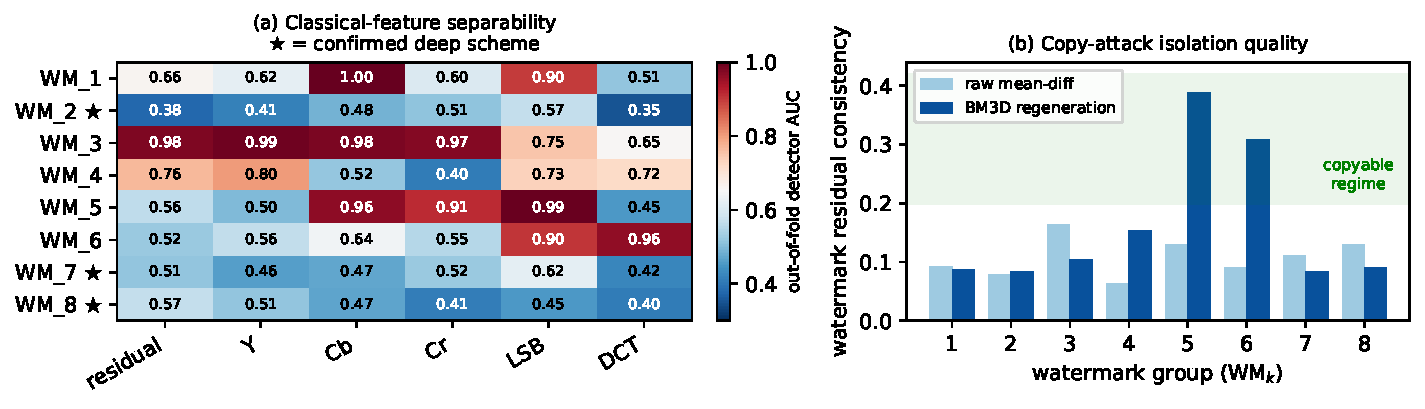
\includegraphics[width=\textwidth]{fig_diagnostics.pdf}
\caption{Diagnostics driving the method. (a) Out-of-fold detector AUC per feature family; rows WM\_2/7/8 ($\star$, later confirmed deep schemes) are near chance everywhere, while the other five light up specific classical features. (b) BM3D copy-attack residual consistency: only WM\_5 and WM\_6 are cleanly copyable additive watermarks.}
\label{fig:diag}
\end{figure}

\section{Evaluation and Results}
Locally, we screened candidates with real LPIPS (matching $S_{\mathrm{qlt}}$ exactly) and, for identification, with source-decode agreement against a clean-image control plus an encode--decode round-trip on the clean targets (the strongest check short of the hidden evaluator). Table~\ref{tab:schemes} reports the three confirmed schemes: each achieves essentially perfect detection at very high quality, exactly the regime the score rewards. Figure~\ref{fig:res}(a) shows the public-leaderboard progression: the two identification steps gave the largest jumps, from $0.334$ (best statistical estimate) to $0.477$ (WM\_2), $0.602$ (WM\_7), and \textbf{0.719245} (WM\_8). The remaining five groups keep their tuned statistical forgeries.

\begin{table}[h]
\caption{Confirmed scheme matches, verified locally. ``Src.\ agree'' is the mean per-bit agreement of the 25 sources' decodes with their majority vote (clean-image control in parentheses); round-trip is bit accuracy after re-embedding the recovered message on clean targets and decoding again; $S_{\mathrm{qlt}}=e^{-8\cdot\mathrm{LPIPS}}$.}
\label{tab:schemes}
\begin{center}
\small
\begin{tabular}{llcccc}
\toprule
Group & Scheme & Message len. & Src.\ agree (ctrl) & Round-trip BitAcc & Mean LPIPS ($S_{\mathrm{qlt}}$) \\
\midrule
WM\_2 & RivaGAN        & 32  & 0.989 (0.626) & 1.000 & 0.0128 (0.903) \\
WM\_7 & TrustMark-Q    & 100 & 1.000 (0.612) & 1.000 & 0.0016 (0.987) \\
WM\_8 & TrustMark-P    & 100 & 0.999 (0.608) & 0.999 & 0.0013 (0.989) \\
\bottomrule
\end{tabular}
\end{center}
\end{table}

\begin{figure}[t]
\centering
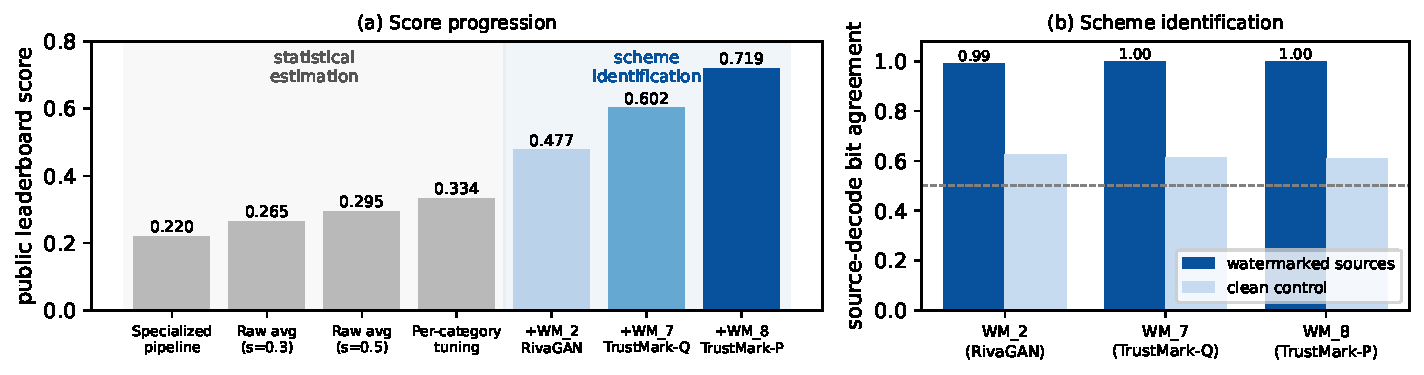
\includegraphics[width=\textwidth]{fig_results.pdf}
\caption{Results. (a) Public score progression; grey bars are statistical estimation, blue bars scheme identification (the decisive gains). (b) Source-decode agreement for the three identified groups: their sources decode almost perfectly under the matched scheme, far above the clean-image control (dashed $=$ chance).}
\label{fig:res}
\end{figure}

\paragraph{Negative results.} Hand-crafted per-domain templates and surrogate+PGD were all beaten by raw averaging (a cross-architecture transfer check showed the PGD surrogates did not generalise); amplitude calibration and denoiser/PCA-subspace/block-statistic estimators did not beat the raw mean-difference --- all consistent with the five unidentified groups having no simple fixed pattern to estimate cleanly. StegaStamp \citep{tancik2020stegastamp} was not pursued: it needs a legacy TensorFlow-1 environment, and Figure~\ref{fig:diag}(a) shows the five remaining groups are classical, not deep, making a deep decoder a low-probability match.

\section{Conclusion}
The final solution forges all eight groups, with the three highest-value ones --- the deep watermarks that classical statistics could not touch --- forged at genuine-encoder fidelity by identifying the underlying open-source scheme (RivaGAN and two TrustMark variants) and re-embedding the recovered message. The best public score was \textbf{0.719245}. The winning insight was diagnostic: the classical-feature AUC map told us \emph{which} groups were deep schemes worth trying to identify versus classical patterns worth estimating.

The practical implication is that invisible watermarking is only as trustworthy as the secrecy and diversity of its embedding. Watermarks now underpin content-provenance systems (e.g.\ labelling AI-generated media). Our attack shows that if an adversary can collect a modest set of images carrying the same message from a known, publicly available scheme, they can recover that message and stamp it onto arbitrary --- including malicious --- content using the real encoder, producing forgeries indistinguishable from genuine provenance. This is exactly the harm the task warns about: a stolen watermark laundered onto attacker-chosen content. Robust deployment therefore cannot treat a decoded watermark as proof of origin; it needs keyed or per-content-secret embeddings, ensembles of undisclosed schemes, detection of re-embedding and copy attacks, and cryptographic signing of provenance rather than reliance on an invisible mark alone.

\small
\begin{thebibliography}{99}
\bibitem[Bui et~al.(2023)Bui, Agarwal, and Collomosse]{bui2023trustmark}
Bui, T., Agarwal, S., and Collomosse, J. TrustMark: universal watermarking for arbitrary resolution images. arXiv:2311.18297, 2023.

\bibitem[Craver et~al.(1998)Craver, Memon, Yeo, and Yeung]{craver1998resolving}
Craver, S., Memon, N., Yeo, B.-L., and Yeung, M. M. Resolving rightful ownerships with invisible watermarking techniques: limitations, attacks, and implications. IEEE JSAC, 16(4):573--586, 1998.

\bibitem[Dabov et~al.(2007)Dabov, Foi, Katkovnik, and Egiazarian]{dabov2007bm3d}
Dabov, K., Foi, A., Katkovnik, V., and Egiazarian, K. Image denoising by sparse 3D transform-domain collaborative filtering. IEEE TIP, 16(8):2080--2095, 2007.

\bibitem[Dong et~al.(2025)Dong, Shuai, Ba, Cheng, Qin, Wang, and Ren]{dong2025wmcopier}
Dong, Z., Shuai, C., Ba, Z., Cheng, P., Qin, Z., Wang, Q., and Ren, K. WMCopier: forging invisible image watermarks on arbitrary images. NeurIPS, 2025.

\bibitem[Kutter et~al.(2000)Kutter, Voloshynovskiy, and Herrigel]{kutter2000copy}
Kutter, M., Voloshynovskiy, S., and Herrigel, A. The watermark copy attack. SPIE Security and Watermarking of Multimedia Contents II, 3971:371--380, 2000.

\bibitem[Sou\v{c}ek et~al.(2025)Sou\v{c}ek, Rebuffi, Fernandez, Jovanovi\'c, Elsahar, Lacatusu, Tran, and Mourachko]{soucek2025transferable}
Sou\v{c}ek, T., Rebuffi, S., Fernandez, P., Jovanovi\'c, N., Elsahar, H., Lacatusu, V., Tran, T., and Mourachko, A. Transferable black-box one-shot forging of watermarks via image preference models. NeurIPS, 2025.

\bibitem[Tancik et~al.(2020)Tancik, Mildenhall, and Ng]{tancik2020stegastamp}
Tancik, M., Mildenhall, B., and Ng, R. StegaStamp: invisible hyperlinks in physical photographs. CVPR, 2020.

\bibitem[Yang et~al.(2024)Yang, Ci, Song, and Shou]{yang2024averaging}
Yang, P., Ci, H., Song, Y., and Shou, M. Z. Can simple averaging defeat modern watermarks? NeurIPS, 2024.

\bibitem[Zhang et~al.(2019)Zhang, Karaman, and Chang]{zhang2019rivagan}
Zhang, K. A., Xu, L., Cuesta-Infante, A., and Veeramachaneni, K. Robust invisible video watermarking with attention (RivaGAN). arXiv:1909.01285, 2019.

\bibitem[Zhang et~al.(2018)Zhang, Isola, Efros, Shechtman, and Wang]{zhang2018lpips}
Zhang, R., Isola, P., Efros, A. A., Shechtman, E., and Wang, O. The unreasonable effectiveness of deep features as a perceptual metric (LPIPS). CVPR, 2018.
\end{thebibliography}

\end{document}
